\chapter{Introduction}
\label{chapter:introduction}
%The histroy of image stitching
The medical imaging technology involves the creation of images of a body part to diagnose the disease in the patient. The advent of digital technology has made the medical image processing easier and very fast. The very fast computing technology helps physician diagnose diseases by real time and automated processing of medical images. This project \emph{``Stitching of X-ray Images''} takes multiple X-ray images of a body part and creates a single, high resolution image. Stitching of medical images is similar to creation of panorama of a scene using several images of a scene. Google has implemented image stitching technology to display the street view of a city~\cite{wiki:google-street-view}.\\

\noindent This report presents the stitching of 2D gray scale medical images; the methods and algorithms can be extended to work for color images too. An X-ray photographic plate is not large enough to fully cover some parts of the body like legs, spines, hands etc. To solve this problem, we capture multiple images of the body part. Then image stitching creates a single high resolution image representing full body part. The single image of the body part makes easy for physicians to diagnose a disease, it is easy to track, manage, store and transmit for electronic medical software.\\

\noindent Algorithms for aligning images and stitching them into seamless photo-mosaics are among the oldest and most widely used in computer vision. Image stitching algorithms create the high resolution photo-mosaics used to produce today's digital maps and satellite photos. They also come bundled with most digital cameras currently being sold, and can be used to create beautiful ultra wide-angle panoramas~\cite{Szeliski:06}. Creating high resolution images by combining smaller images are popular since the beginning of the photography~\cite{Kumar:10}.\\

\noindent There should be nearly exact overlaps between images for stitching and identical exposures to produce seamless results~\cite{Ward06:3}. The stitching is not possible if there is not any common region between images. The images of same scene will be of different intensities, scale and orientation and stitching should work or at least give visually appealing output. \\

\noindent Several algorithms are there to accomplish image stitching, but no algorithm is guaranteed to work with 100\% accuracy. The traditional algorithms carry out pixel wise registration (\emph{exhaustive method}) which use some error criteria to get the best result i.e. the best registration is the one which gives least error value. Those methods are slower and sometimes there is chance of not giving the best result. The feature based registration methods find distinctive features in each image and then efficiently match to rapidly establish correspondences between pairs of images to determine the approximate \emph{motion model}. Feature-based approaches have the advantage of being more robust against scene movement and are potentially faster, if implemented the right way\cite{Szeliski:06}. The common feature points are used to create the relationships between the images which makes them suitable for automated stitching.\\

\noindent This first section of this chapter gives introduction to X-ray imaging; describes how X-ray images are produced and their characteristics. The following sections discuss the various types of image alignment methods and the overall stitching process. The challenges of the image stitching have been discussed in the last section. 

\section{X-Ray Imaging}
The X-ray technology was developed in 1895 by \textit{Wilhelm Roentgen}, a German physicist. X-rays are produced by changing the energy state of electrons. The highly accelerated electrons are decelerated by bombarding on a metal block. The interaction of electrons in metal block change the energy state releasing X-rays. The X-rays production process is shown in figure~\ref{fig:x-ray-tube}.\\

\begin{figure}%
\centering
\subfloat[X-ray Tube]{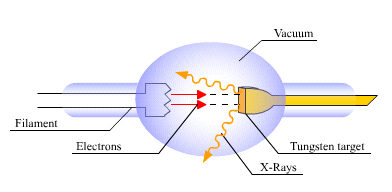
\includegraphics[width=0.7\columnwidth]{2.mainmatter/1.Introduction/figures/x-ray-tube}\label{fig:x-ray-tube}}%
\subfloat[X-ray image of Chest]{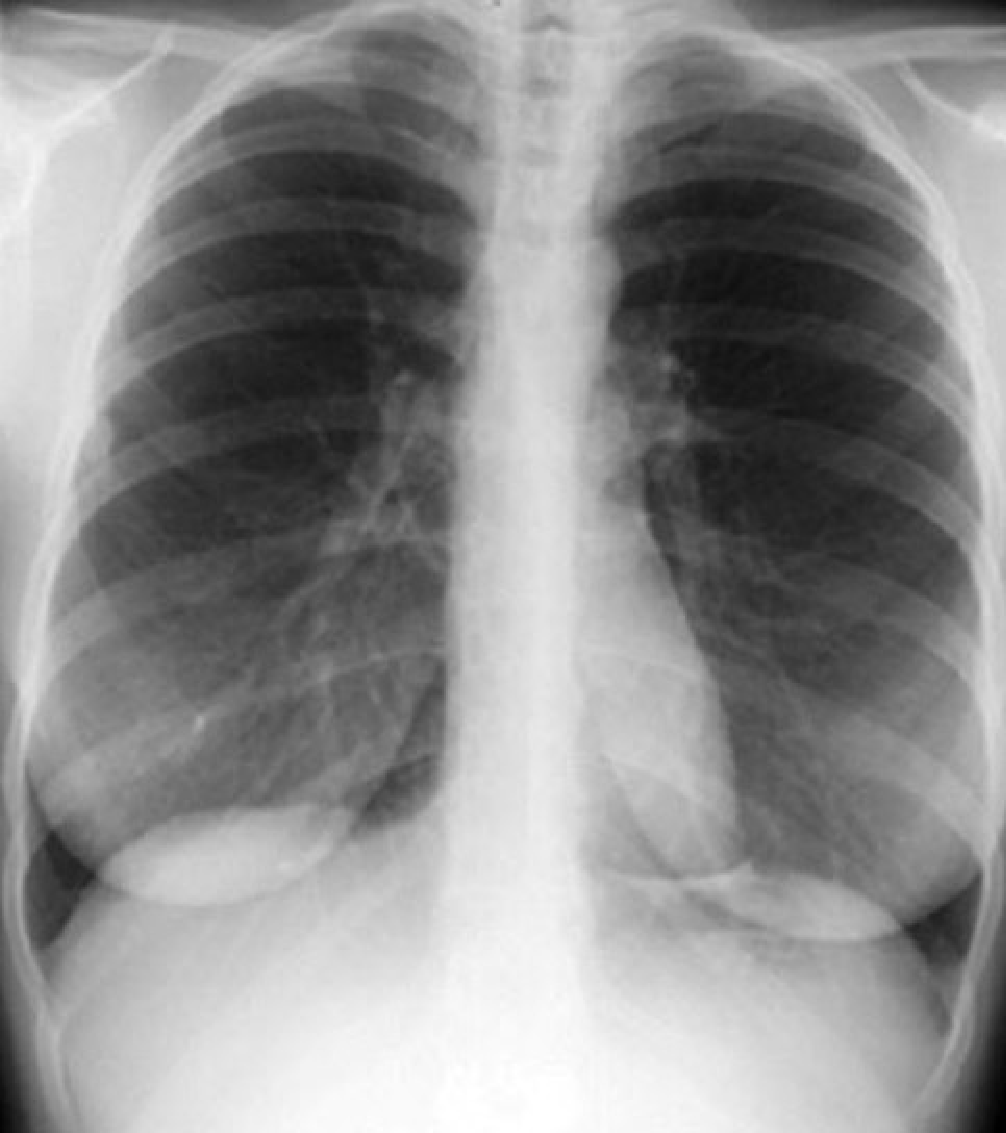
\includegraphics[width=0.3\columnwidth]{2.mainmatter/1.Introduction/figures/chest-x-ray}\label{fig:x-ray-image}}
\caption[Production of X-ray]{Production of X-ray:~\subref{fig:x-ray-tube} is X-ray tube used to produce X-ray images.~\subref{fig:x-ray-image} is a sample X-ray image.}
\end{figure}
\begin{description}
\item[Flat Panel Receptors] The X-rays can penetrate soft body parts and go into the bones, so X-ray images are used to view and analyze inner body parts for pathology. X-rays are detected by using \textit{image receptors (IR)}. The new digital technology has been replacing the old technology which uses films and chemicals to store X-ray images. The \emph{Flat Panel Receptors} stores the X-ray images digitally and those digital X-ray images are portable i.e. they can easily be available in multiple places. We can use computer-assisted diagnosis methods to digital X-ray images. Figure~\ref{fig:x-ray-system} shows an X-ray machine which consists of X-ray generator and flat panel receptor. The body is placed in between the X-ray source and receptor so that it can penetrate the body part. The X-rays which pass through the body part are stored in the receptor.
\end{description}

\begin{figure}%
\centering
\subfloat[]{
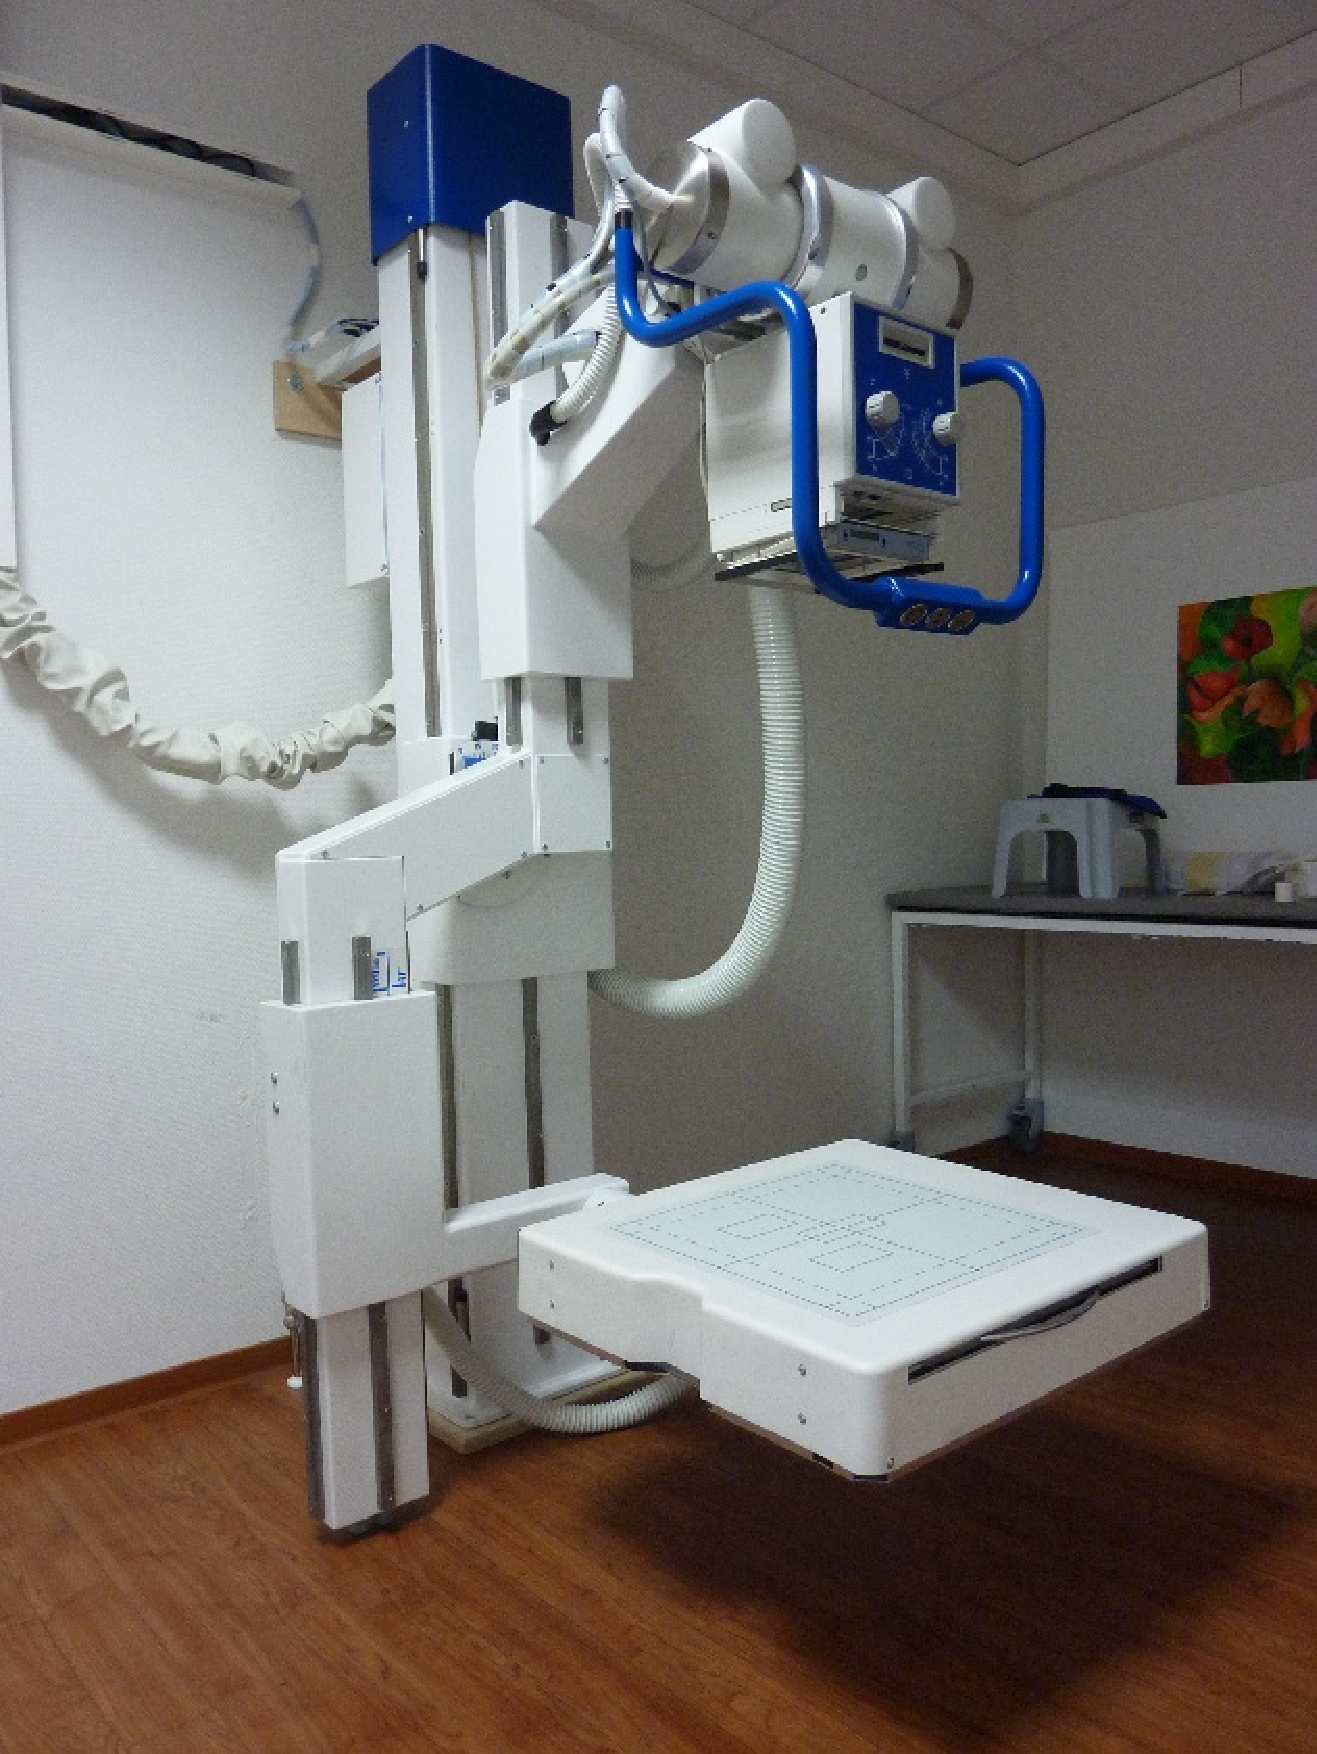
\includegraphics[width=0.5\columnwidth]{2.mainmatter/1.Introduction/figures/X-ray-machine}%
\label{fig:x-ray-machine}
}%
\hspace{8pt}
\subfloat[]{
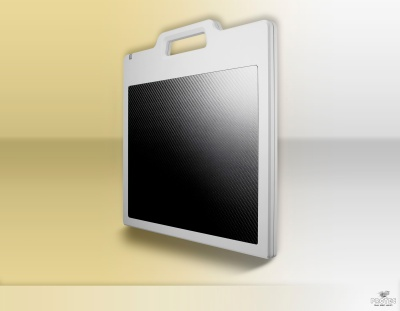
\includegraphics[width=0.4\columnwidth]{2.mainmatter/1.Introduction/figures/flat-panel}
\label{fig:flat-panel}
}%
\caption[X-ray Imaging System]{X-ray Imaging System.~\subref{fig:x-ray-machine} X-ray Machine~\subref{fig:flat-panel} Flat Panel \tiny({Image source: http://www.protec-med.com})}
\label{fig:x-ray-system}
\end{figure}

\noindent X-ray images are negative images i.e. dense object like bone or metal fragments display brighter while the soft parts look darker. The X-ray images depicts all the object's features inside and out, so a point in an x-ray image is the summation of shadows; while general photograph shows only object's surface. In other words, the brightness of a point in the film is the summation of all the densities the ray encountered~\cite{Durnavich:00:online}.\\ 

\begin{itemize}

	\item{\textit{Scaled and Oriented X-ray Images}} Since the X-ray tube is movable, the distance of the tube to the body part determines the scale of the image. When X-ray tube is very near to the patient, the image will be distorted because of magnification. Similarly, when X-ray tube is rotated laterally, we get perspective images. We get rotated images because of mobile patient table. 
	
	\item{\textit{Density of X-ray images}} The density of X-ray image is  the overall blackness or darkness of the film. The flesh, or soft tissue is the least dense and therefore allows for the x-ray to pass easily to the film. Many X-ray photons interact with the film causes the density on the film to black. So, thickness of the body part is inversely proportional to the density of the film. The exposure time, operative voltage peak and current also control the density i.e. if operating voltage and current increases, film density also increases. The overexposed film has a high density, blackens the film and underexposed film has low density means it is white.
	
\item{\textit{Contrast of X-ray images}} The contrast of X-ray image depicts the difference in degree in blackness between adjacent areas. The image with low contrast contains many shades of gray while high contrast image consists of very dark and very light areas. X-ray contrast is produced because X-ray penetration through an object differs from the penetration through the adjacent background tissue. The radio-graphic recording system should be able to fully record all the contrast in the X-ray image~\cite{Sprawls:online}.
\end{itemize}






\section{Pixel Based Alignment}
Before stitching is carried out, two images need to be aligned properly so that the same region in the images overlap each other. Pixel based alignment methods are classical methods which carry out pixel-wise comparison of the two images. We shift or warp images relative to each other and look at how much the pixels agree. The pixel-to-pixel matching methods are also called direct methods. We use suitable error metric (section 3.6) and we carry out exhaustive search for all possible alignments to get optimal alignment. This is very slow process; so hierarchical coarse-to-fine techniques based on image pyramids can be used to make it faster~\cite{Szeliski:06}.




\section{Feature Based Alignment}
The pixel based alignment methods are not appropriate for real time image stitching applications which includes large (i.e. high resolution) X-ray images. So, \emph{feature based alignment} methods are selected to get faster stitching. The feature based method extract the distinctive features from each image to match those features to establish global correspondence and then estimate the geometric transformation between the images~\cite{Szeliski:06}. Interest points (corners) in the image are selected as feature points and the feature descriptors are extracted for each point. The feature descriptors describe the point and for matching process, those descriptors should be invariant to image rotation, scaling or even intensity variations. To find the matching points, the points in one image are compared to the point in another image, an appropriate distance measure is implemented to find out the similarity between the points, and matching pairs have the minimum distance between them. 

%Image Stitching Process
\section{Image Stitching Process}
In this section, I will describe the fundamental steps of image stitching. Image stitching system gets two or more images as input and the output will be a single stitched image. The image stitching process can be divided into 5 sub-processes mentioned below:
\begin{description}
\item [\textit{Feature detection}]
This step gets the input images\footnote{input images should be already preprocessed by noise reduction, intensity leveling etc.} and features of the images are extracted. The important points (also called \textit{key points} or \textit{corners}) in the image are identified using one of the corner detection methods. The concept of corner detection will be discussed in section~\ref{sec:corners-in-image}. Each feature point will have unique descriptor which is used for feature matching.   

\item [\textit{Feature matching}]
After we get a number of feature points in the images, the next step is to match the feature points. The similar points in the images are identified using one of the feature matching techniques. %[section~\ref{sec:feature-matching}].
The feature matching step gives the best matching point pairs between the images which are used for estimation of motion parameters.

%\begin{figure}%
%\includegraphics[width=\columnwidth]{2.mainmatter/1.Introduction/figures/stitching-flowchart}%
%\caption{Image Stitching Flow Chart}%
%\label{fig:stitching-flowchart}%
%\end{figure}



\item [\textit{Motion estimation}]
Based on the matching points, we estimate the motion parameters (like transformation, rotation or scale parameters). To estimate the motion parameters, we need true matched points. The false matching points gives wrong motion parameters which produce incorrect alignment. We create a mathematical model with the motion parameters, and the best model is selected which represents most of the matched points (RANSAC) or gives least error value (LMS) as described in chapter~\ref{chapter:homography-estimation}.   
 
\item [\textit{Transformation}]
After we estimate the motion parameters, the next step is to transform the image. The transformation includes translation, rotation, scaling or perspective transform. After transformation, we get the aligned image with overlapping areas lying on the same location of the composite image.  
\item [\textit{Blending}]
This is final step of image stitching. If the overlapping areas are not exact\footnote{The overlapping areas are never exact in real problems}, we get visible lines (seams) in the composite image. So, we use blending techniques to remove those discontinuities. The blending techniques have been discussed in chapter~\ref{chapter:compositing}.
\end{description}



\section{Challenges of Image Stitching}
Image stitching, in real life medical applications, consists of several challenges to get the better result. The stitching system should be able to work or to some extent give better output result for medical images. In this section, I am going to highlight some of the challenges of image stitching.
\begin{description}
  \item [\textit{Image Noise}]{If image is noisy, there may be chances that stitching methods fail to give accurate result. So, we have to implement some mechanism as pre-processing to suppress or remove the noise to get the better result. The corner-based stitching methods are very sensitive to noise because they give a lot of false corner-points.}
	\item [\textit{Computational Time}]{The stitching methods are slower, if we don't optimize the methods, it takes a lot of time to get the result because of heavy computation (feature based methods) or lengthy process (direct methods) required. The high resolution images contain a lot of pixels in the image, so, the direct methods require a lot of time to align the methods. The feature based methods require heavy computation to get and match the features in the image. The optimization of the methods should be done in such a way that it results acceptable accuracy (trade-off between computational-complexity and accuracy)}
	\item [\textit{Intensity Variation}]{Some image stitching methods are very sensitive to variation image intensities resulting inaccurate stitching. Again, intensity variation in images causes problem in blending also because it creates a seam line in the join of the image.}
	\item [\textit{Image Orientation}]{The images to be stitched need not necessarily in same orientation. The rotation, scaling, distortion between images should be covered by the stitching methods i.e. the stitching methods should give accurate result for rotated, scaled or distorted images.}	
\end{description}

%Related Work
\chapter{Related Work}
%Describe all the related works
%Exhaustive Matching
%Chamfer Matching
%Will be intensive articles oriented.
%Harris Corner Detection
%Pattern based matching
%SIFT Corner Detectors
%SURF Corner Detectors
% OpenCV library
This chapter surveys previous work in image stitching. As already said in chapter~\ref{chapter:introduction}, algorithms for aligning images and stitching them into seamless photo-mosaics are the oldest and most widely used in computer vision. The first image stitching concept was known to be implemented to create panoramas in 1787 by \emph{Robert Barker}, an Irishman, who created panoramas of a cylindrical building~\cite{Woeste:09}.\\

\noindent In the past, exhaustive methods were used which calculate a measure of the difference between the images at all possible values in the search space. Those methods were time consuming. If we are registering two images: $I_1$ of size $M X M$ and $I_2$ of size $N X N$, then the computation complexity will be $O(M^2N^2)$ \footnote{matching for rotated images,complexity increases.}.Those methods were used for long time until \emph{Lucas and Kanade}'s patch-based translational alignment\cite{Lucas:81}. The registration method purposed by Lucas and Kanade~\cite{Lucas:81} became widely popular at that time because it drastically reduced the computational time to $O(M^2 log N)$. The matching process was an iterative \emph{Newton Raphson} method where we go on getting better match in each iteration. \\ 

\noindent Similarly, \emph{Xue Mei} and \emph{Fatih Porikli}~\cite{Mei:06} have purposed a computationally inexpensive method for multi-modal image registration. Their method employs a joint gradient similarity function that is applied only to a set of high spatial gradient pixels. They used the gradient ascent method to get the maximization of similarity function which gives the motion parameters for best match. \\ 

 

\noindent The edge based \emph{Chamfer matching} methods also became popular which used the edge information in the image for matching. In Chamfer matching, we select an image as template and try to match with other image using distance transform as shown in figure~\ref{fig:matching-dt}. We can use the various transformed templates to match rotated images~\cite{Gavrila:98}. Gavrilla and Philomin~\cite{Gavrila:99} implemented the Chamfer based matching method in real-time detection of traffic signs and pedestrians from a moving vehicle. They used coarse-to-fine approach over the shape hierarchy and over the transformation parameters to make the matching faster.\\ 

\begin{figure}%
\begin{center}
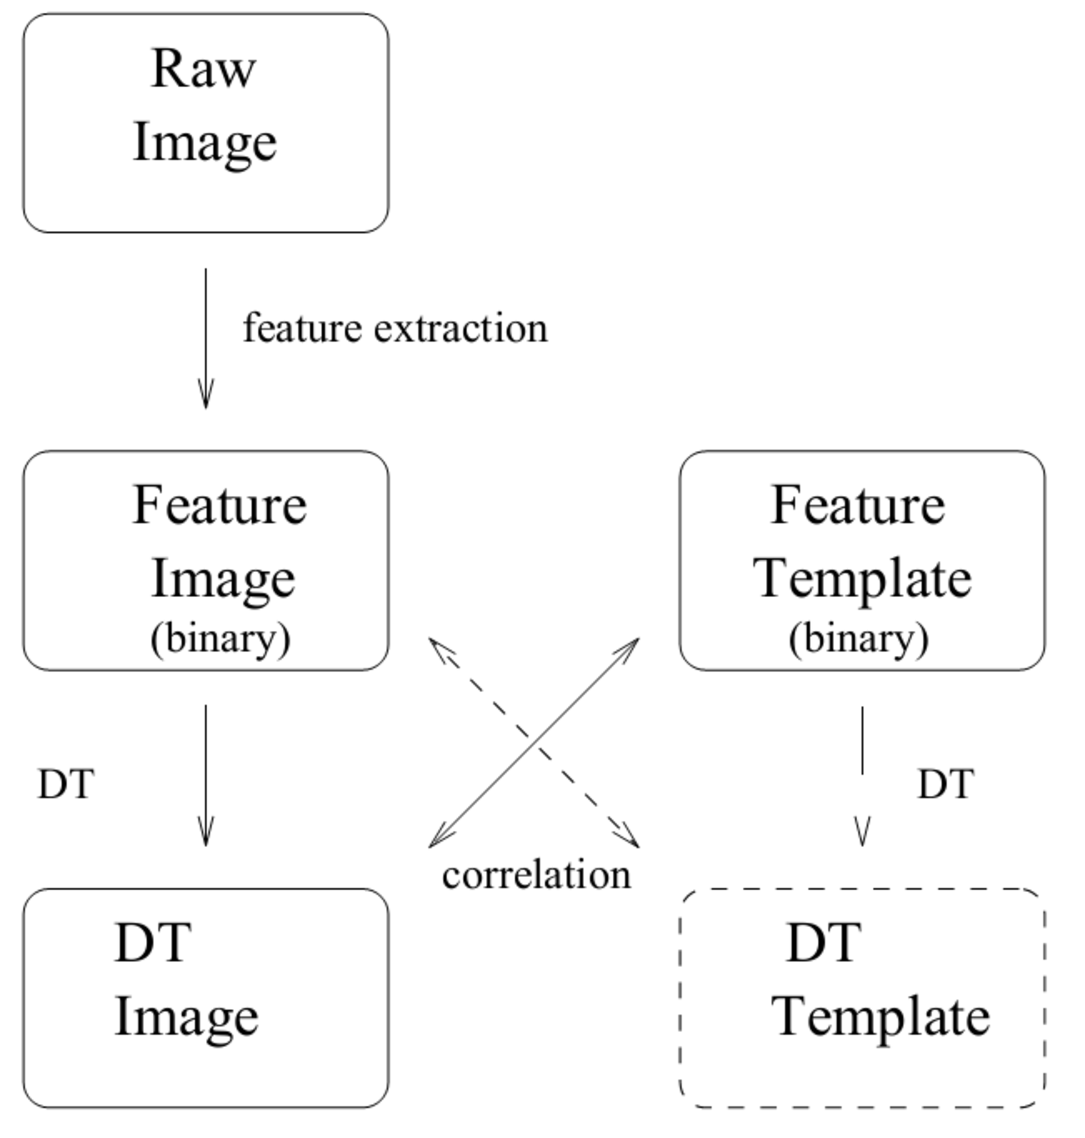
\includegraphics[width=0.5\columnwidth]{2.mainmatter/1.Introduction/figures/chamfer-matching}%
\caption[Matching Using a DT]{Matching using a distance transform. \imgsrc{(Image source: Gavrilla~\cite{Gavrila:98})}}%
\label{fig:matching-dt}%
\end{center}
\end{figure}

\noindent There are several research papers which describe the global image alignment methods. The computation of globally consistent alignments has been discussed in the literature by Szeliski and Shum~\cite{Szeliski:97} and the variations of exposure has been addressed by Sawhney \textit{et al}~\cite{Sawhney:99}.\\ 


\noindent More recent algorithms on image alignment extract a sparse set of feature points and match these points to each other to get the motion parameters~\cite{Szeliski:06}. \emph{Brown} and \emph{Lowe} in their paper~\cite{Brown:02} discusses on obtaining the invariant local features to find the matches between the images and they also claim the method to be insensitive to ordering, orientation, scale and illumination of input images. And there are several research papers which discuss on extracting the feature points in the image. Some basic corner detectors including \emph{Harris} have been discussed by Parks and Gravel~\cite{Parks:11}. Similarly, the very fast corner detector(\emph{Features from Accelerated Segment Test}) have been purposed by Rosten et al~\cite{Rosten:06}. The more robust feature points extractors (\emph{SIFT} and \emph{SURF}) has been discussed by Lowe~\cite{Lowe:04} and Bay et al~\cite{Bay:08}. The authors of the papers claim that those feature extractors are more robust and invariant to image rotation, scale or intensity changes. 





 
%Background Theory
\chapter{Background Theory}
There are some basic mathematical and image processing principles that we need to be familiar before we start image stitching. In this chapter, we basically focus on 2D gray scale image processing and its not a big deal to extend the methods for colored images. 
\section{Image Representation}
An image consists of information and that should be represented in a form of data structure. This section discusses two main data structures used in image analysis applicable for this thesis project.
\subsection{Matrices}
In matrix representation, each pixel of the image is represented in the form of matrix. The binary images are represented by a matrix containing only zeros and ones. For N-bit gray scale images, the matrix contains the values from 0 to $2^N-1$. Figure~\ref{fig:image_matrix} shows 8-bit gray scale image in matrix form.\\

\noindent The multispectral images contain multiple matrices to represent each spectrum (e.g. RGB color images are represented by 3 matrices containing red, green and blue values). All matrix related operations (like addition, subtraction, multiplication, scaling, inverse etc.) can be applied to the images represented in matrix form. 
\begin{figure}[t]%
\begin{center}
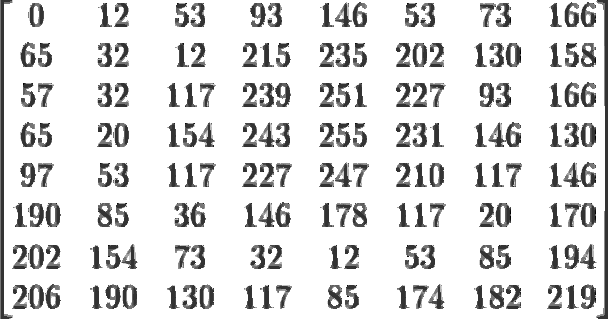
\includegraphics[width=0.6\columnwidth]{2.mainmatter/1.Introduction/figures/matrix_image}%
\caption[Image in Matrix Form]{Image represented in matrix form.The elements matrix are the pixel values}%
\label{fig:image_matrix}%
\end{center}
\end{figure}

 % Refer to Ps. 99 Sonka
\subsection{Pyramids}
\label{subsec:pyramids}
% Refer to Ps. 106
Processing higher resolution images is time consuming and are not suitable for interactive system design. So, to make it faster, we process the images in lower resolution to select the interesting parts in image and further processing is carried out to the selected parts in higher resolution~\cite{Sonka:08}.
\begin{figure}[!tb]
\begin{center}
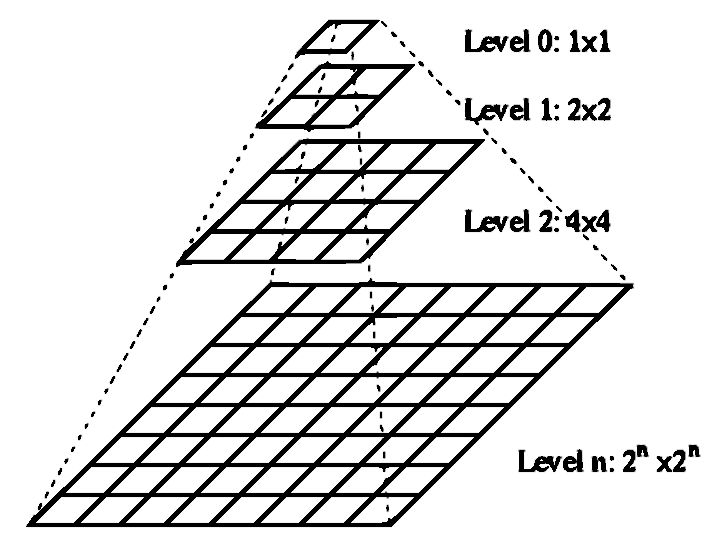
\includegraphics[width=1\textwidth]{2.mainmatter/1.Introduction/figures/Image_Pyramid}%
\caption[Image Pyramids]{Image Pyramids. \imgsrc{(Image source: http://fourier.eng.hmc.edu)}}%
\label{fig:pyramids}%
\end{center}
\end{figure}
This is achieved by generating matrix pyramids of an image which consists of a sequence of images $\{M_L,M_{L-1},...,M_0\}$ (figure~\ref{fig:pyramids}) where $M_L$ has the same dimension and elements as the original image and $M_{i-1}$  will have half resolution of $M_i$. We can create image up to $M_0$ (i.e. 1 pixel) if we have square image with dimension multiple of 2. Generally, we will select a level and generate the pyramid of images up to that level. The level to be selected depends upon the specific problem.\\

\noindent There are two types of pyramids: low-pass pyramids and band-pass pyramids. In low pass pyramid, we smooth the image with appropriate smoothing filter, and sub sample the smoothed image to create smaller image.\footnote{Gaussian pyramid is created using Gaussian smoothing filter. If we go from bottom to top, in each level, the image size is reduced by $\frac{1}{2}$} Band pass pyramid, on the other hand, is obtained by creating the difference between the adjacent levels in the pyramid. To compute pixel-wise differences, the size of the images should be same, so, we have to implement some interpolation or scaling techniques.


\section{Brightness Transformation}
Brightness transformation is carried out to make the images look more clearer. In brightness transformation, the intensity of the image pixels are changed using one of the following methods:
%Brightness Thresholding
\begin{description}
\item[Brightness Thresholding]
We select an intensity value P and then the image pixels with intensity less than p are set to zero and other pixels are set to 1 resulting black-and-white image. 

\item[Histogram Equalization]
Histogram equalization is used to enhance contrast by creating an image with equally distributed brightness levels over the whole brightness scale. If an image consists of pixels with limited level of intensities, then the histogram equalization assigns all range of intensities to the pixels which results increase in contrast. For algorithm, please refer to the book by Sonka \textit{et al}~\cite{Sonka:08}.

\begin{figure}%
\centering
\subfloat[]{%

\includegraphics[width=0.3\columnwidth]{2.mainmatter/1.Introduction/figures/gray_scale_original}%
\label{fig:gray_image}%
}%
\hspace{8pt}%
\subfloat[]{%

\includegraphics[width=0.3\columnwidth]{2.mainmatter/1.Introduction/figures/gray_scale_equalized.pdf}%
\label{fig:hist_trans_image}%
}%
\caption[Histogram Transformation]{Histogram Transformation:
	\subref{fig:gray_image} is original image;
	\subref{fig:hist_trans_image} is histogram transformed image.}%
\label{fig:hist_trans}%
\end{figure}

%\subsection*{Logarithmic Gray-scale Transformation}


\item[Look-up Table Transformation]
Look-up table is used to transform brightness in real time. The transformation information of all possible gray levels is stored in look-up table, and the transformation is carried out using the table. For example, 8 bit image contains 256 gray levels and only 256 bytes of memory is required for look-up table. 
\item[Pseudo-color Transformation]
The brightness of the pixels are represented by some color value to perceive more detail information. Also human eye is more sensitive to color change than brightness change. 
\end{description}

\section{Geometric Transformation}
In geometric transformation, we use a vector function \emph{T} which maps the pixel (x,y) to a new position (x',y') defined by the following two component equations:
\begin{equation}
x'=T_x(x,y), y'=T_y(x,y)
\label{eq:geom-trans}
\end{equation}
The transformation vector function \textbf{T} known in advance or sometimes we calculate from original and transformed images by matching of the corresponding pixels. 

\subsection*{Pixel Co-ordinate Transformation}
The co-ordinates of the input image pixels are mapped to the point in the output image. The geometric transform can be classified as
\begin{itemize}
	%\item {\textit{Bilinear Transform}} The bilinear transform is represented by:
	%\begin{equation}
	%\begin{array}{lcl}
	%x' & = & a_0+a_1x+a_2y+a_3xy,\\	
	%y' & = & b_0+b_1x+b_2y+b_3xy
	%	\end{array}	
	%\label{eq:bilinear-trans}
	%\end{equation}
	%For bilinear transform, we need four pairs of corresponding points.
	
	\item {\textit{Affine Transform}}
	The affine transform is simple and only 3 pairs of corresponding points are sufficient to find the coefficients.
	\begin{equation}
	\begin{array}{lcl}
		x' & = & a_0+a_1x+a_2y,\\
		y' & = & b_0+ b_1x+ b_2y
	\end{array}
	\label{eq:affine-trans}
	\end{equation}
	The affine transform consists of rotation, translation, scaling and skewing. 
	
	\item {\textit{Perspective Transform}}
	The perspective transform also called \emph{homography} denoted by a 3 x 3 matrix \textit{H} and the transformation is carried out as:
	\begin{equation}	
		x'  =  \frac{h_{00}x+h_{01}y+h_{02}}{h_{20}x+h_{21}y+h_{22}} \mbox{ and } 
		y'  =  \frac{h_{10}x+h_{11}y+h_{12}}{h_{20}x+h_{21}y+h_{22}}	
	\label{eq:perspective-transform}
	\end{equation}
	The perspective transforms preserve straight lines and are appropriate for 3D scenes observed under pure camera rotation or planes observed under general 3D motion~\cite{Szeliski:06}. We need four pairs of corresponding points for perspective transform.
	
	%\begin{figure}%
	%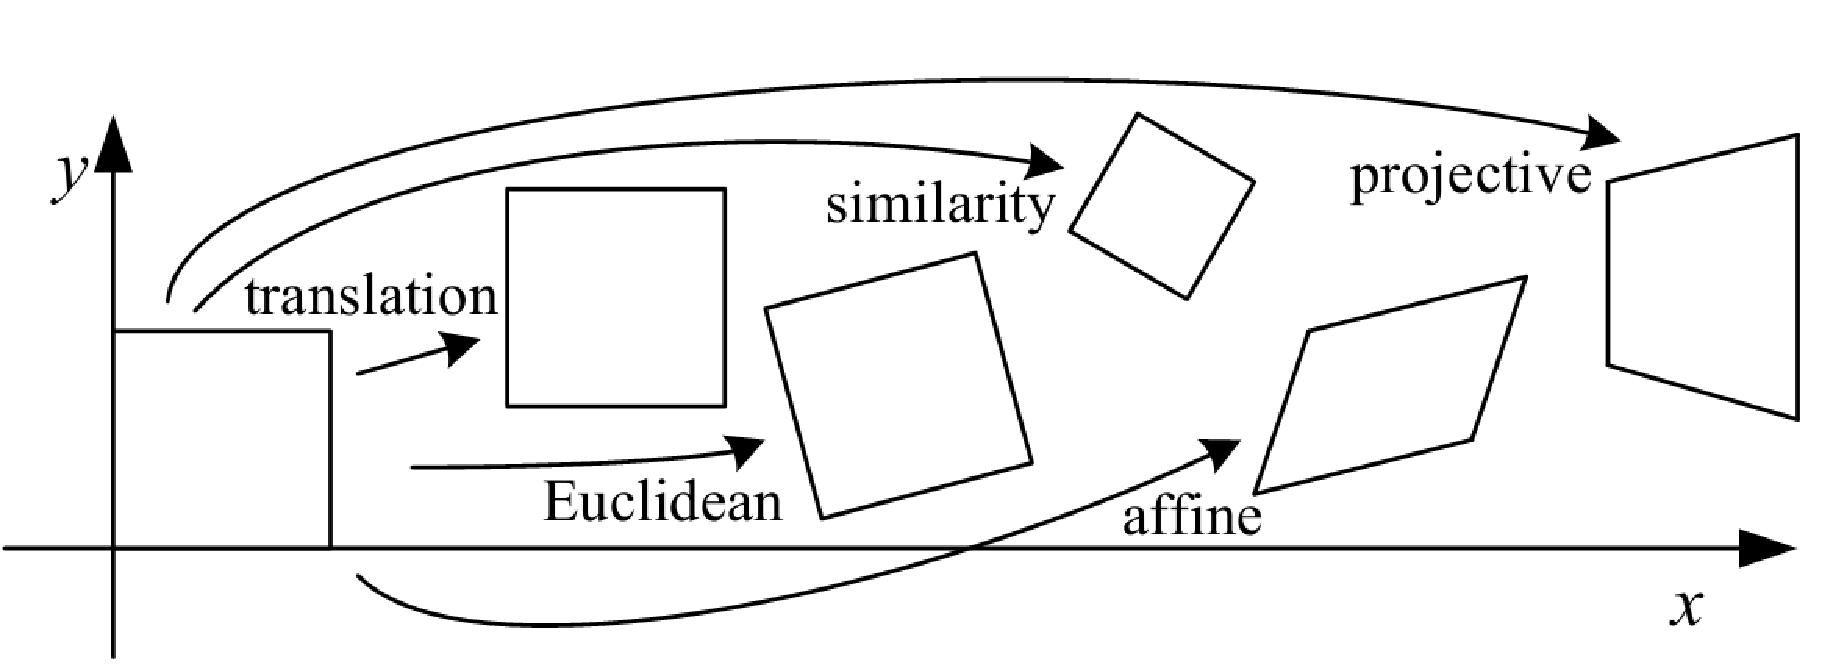
\includegraphics[width=\columnwidth]{2.mainmatter/1.Introduction/figures/2D-planar-transformation}%
	%\caption[Basic 2D Planar Transformation]{Basic 2D planar transformation. Image source:\cite{Szeliski:06}}%
	%\label{}%
	%\end{figure}
	
\end{itemize}

\subsection*{Brightness Interpolation}
The transformation generally results the continuous co-ordinate values (real numbers). The intensity value of specific integer grid in the output image is set by interpolating the brightness of neighboring non-integer samples. Brightness interpolation influences image quality. The simpler the interpolation, the greater is the loss in geometric influences and photometric accuracy~\cite{Sonka:08}. The most common interpolation methods are \emph{nearest neighbor}, \emph{linear} and \emph{bi-cubic}.

\section{Image Smoothing}
\label{sec:image-smoothing}
% Refer ps. 125
If an image contains a lot of noise, we need to have proper mechanism to reduce the noise using image smoothing methods. Generally, smoothing methods blur the edge information, so if we need to preserve the edge information, then we have to implement ``\textit{edge preserving}'' image smoothing methods. 
\subsection*{Averaging}
The noise present in the image at each pixel is an independent random value with zero mean and standard deviation $\sigma$. So, if we could get n images of the same static scene, we estimate the average of the images to remove out the noise. It is to be noted that for averaging, we need more than one images of the same scene.

\subsection*{Median Filter}
The median filter is very effective noise reduction technique because if we use it appropriately, it can reduce the noise while preserving the edge information~\cite{Donoho:09}. The median value is chosen from the pixels defined by kernel window, and since this process is carried out all the pixels in the image, it is slower method for high resolution image. Median filter is very widely used in digital image processing to remove \emph{speckle noise} and \emph{salt \& pepper noise}.  

\subsection*{Gaussian Filter}
In Gaussian filter, the image is convolved with the Gaussian function to reduce image noise. In digital image processing, a kernel window defines the effective neighborhood pixels. So, larger window size creates more blurred image. Fourier transform of a Gaussian function is another Gaussian, so Gaussian blur has the effect of reducing the high frequency components (i.e. low pass filter). \\
\begin{equation}
L(x,y,\sigma)=G(x,y,\sigma)* I(x,y)
\label{eq:gaussian_blur}
\end{equation}
where * is the convolution operation in $x$ and $y$, and 
\begin{equation}
G(x,y,\sigma)=\frac{1}{2 \pi \sigma^2} e^{-\frac{(x^2+y^2)}{2 \sigma^2}}
\label{eq:gaussian-function}
\end{equation}

\noindent Apart from smoothing, Gaussian filter can be used to generate different scales of an image as a processing stage in computer vision algorithms. For higher resolution images, the processing on original images might be complicated, so lower resolution scaled image is used for simplicity (section~\ref{subsec:pyramids}).\\

\noindent The derivative based edge detectors are sensitive to noise, so Gaussian blur filter is commonly used before the edge detection algorithm is carried out. This is called \emph{Laplacian of Gaussian} or \emph{LoG} filtering.

\section{Edge Detection}
\label{sec:edge-detection}
The edge detectors are very important in computer vision which helps for image understanding and perception by finding lines, region boundaries etc. Edges are detected by identifying the intensity changes in the image; edges are the pixels in the image where intensity changes abruptly. Edge detection is opposite to smoothing; in smoothing we remove high frequency components while in edge detection, we remove low frequency component in the image. \\

\noindent Edge detection is not a trivial task; we can not create a general edge detector working for all types of images. Generally, edge detectors work approximating the derivative (first or second order) of the image function. There are some operators such as \textit{Roberts}, \textit{Sobel}, \textit{Prewitt}, etc. which approximate the first order x- and y- derivatives of the image and calculate the resulting magnitude and direction of the edges. The alternative methods of edge detection use second derivative of the image function and the edge pixels will be the zero crossings of the second derivative.\\

\noindent The above mentioned derivative based methods are very sensitive to the noise in the image~\cite{ziou:98}~\cite{lindegerg:96}. So, we have to implement some noise reduction mechanism before differentiation of image is carried out. 

\subsection{Laplacian of Gaussian}
Before we compute the image derivative, we convolve the image with Gaussian filter to suppress the noise present in the image. Suppose, $f(x,y)$ be image function, $G_\sigma(x,y)$ be the Gaussian kernel of width $\sigma$, then
\begin{equation}
\Delta [G_\sigma(x,y) \otimes f(x,y)]=[\Delta G_\sigma(x,y)] \otimes f(x,y) = LoG \otimes f(x,y)\\
\label{eq:LoG1}
\end{equation}
where
\begin{equation}
LoG=\frac{x^2+y^2-2\sigma^2}{\sigma^4}e^{\frac{-(x^2+y^2)}{2\sigma^2}}
\label{eq:LoG2}
\end{equation}

\noindent Thus, from above equation, we conclude that Laplacian operator to the Gaussian smoothed image is equivalent to applying \emph{Laplacian of Gaussian (LoG)} operator to the original image. 

\subsection{Approximation with Difference of Gaussian}
The Laplacian of Gaussian (LoG) can be efficiently implemented using \emph{Difference of Gaussian (DoG)} at different scales. Suppose we used Gaussian kernels $G_{\sigma1}$ and $G_{\sigma2}$ to get smoothed images $g_{\sigma1}(x,y)$ and $g_{\sigma2}(x,y)$, then
\begin{equation}
g_{\sigma1}(x,y)-g_{\sigma2}(x,y)= (G_{\sigma1}-G_{\sigma2}) \otimes f(x,y)=DoG \otimes f(x,y)
\label{eq:DoG}
\end{equation}
\begin{figure}%
\centering
\includegraphics[width=1.0\columnwidth]{2.mainmatter/1.Introduction/figures/DoG-Log}%
\caption[Comparison of DoG and LoG]{Comparison of DoG and LoG. \newline \quad \imgsrc{(Image source: http://en.wikipedia.org/wiki/Difference\_of\_Gaussian)}}%
\label{fig:DoG-LoG}%
\end{figure}
\noindent The comparison graph in figure~\ref{fig:DoG-LoG} shows the similarity between DoG and LoG operators. Thus, we can approximate Laplacian of Gaussian by simply subtracting the Gaussian blurred images in different scales. 

\section{Error Metrics}
Error metrics give the measurement of similarity between two images. So, in registration process, we try to align the two images that gives optimal error value. The direct methods of image matching choose a suitable error metrics to compare the images~\cite{Szeliski:06} and the search process will try to get the optimal error value. 
\subsection*{Sum of Squared Differences}
The sum of squared differences (SSD) gives the dissimilarity measurement between two images. So, in alignment process, we try to minimize the SSD value which is calculated as follows:
\begin{equation}
E_{SSD}=\sum_{i}{[I_1(x_i)-I_0(x_i)]^2}=\sum_{i}{e_i^2}
\label{eq:ssd}
\end{equation}
where $e_i=I_1(x_i)-I_0(x_i)$ is \emph{residual error}.

\subsection*{Correlation}
The cross-correlation of the two aligned images are calculated,
\begin{equation}
E_{CC}=\sum_{i}{I_0(x_i)I_1(x_i)}
\label{eq:cross-cor}
\end{equation}
The cross-correlation value between two images does not give accurate result in case when a very bright patch exists in one of the images~\cite{Szeliski:06}. So, \emph{Normalized Cross-Correlation} (NCC) is commonly used,
\begin{equation}
E_{NCC}=\frac{\sum_{i}{[I_0(x_i)-\overline{I_0}] [I_1(x_i)-\overline{I_1}]}}{\sqrt{\sum_{i}{[I_0(x_i)-\overline{I_0}]^2[I_1(x_i)-\overline{I_1}]^2}}}
\label{eq:}
\end{equation}
where 
\begin{equation}
\overline{I_0}=\frac{1}{N}\sum_{i}{I_0(x_i)}  
\label{eq:}
\end{equation}

\begin{equation}
\overline{I_1}=\frac{1}{N}\sum_{i}{I_1(x_i)}
\label{eq:}
\end{equation}
The NCC value 1 indicates the two images are exactly same. To get the best alignment, we transform the image in such a way that it gives maximum NCC value.

\subsection*{Key Points Matching}
The key-points (feature points) between the images are identified by using some key-point detectors. We implement matching algorithm to get the matching points. The points which do not get any matching point are counted for both the images to measure the dissimilarity between the images. For perfectly matching images, the count will be zero implies the images are same. The larger the number of count, the more dissimilarity between the images.

\section{Corners in Image}
\label{sec:corners-in-image}
%Refer Sonka 157 and others
The geometric transformation parameters are estimated using the position of corresponding points. The same transformation generally hold for almost all pixels of the image and the necessary number of corresponding pairs of points is usually rather small and is equal to the number of parameters of the transformation. The same transformation usually holds for almost all pixels of the image. We have to examine all possible pairs of pixels to find out the correspondence and this is computationally expensive. If two images have n pixels each,the complexity is O($n^2$). So, to simplify this problem, we find out the \emph{interest points (corners)} and those interest points are used to find out correspondences for estimation of transformation parameters. The corner in the image can be defined as a pixel in its small neighborhood where there are two dominant and different edge directions\cite{Sonka:08}. The number of interest points are much smaller than the pixels in the image, so it greatly reduces the computational complexity.\\

\noindent The corner detectors generally use the gray scale image as input and do some processing and the final result is an image with pixel values proportional to the likelihood of the corner and we use thresholds to find out the corner points. We can get the required number of interest points by using proper threshold. Corner detectors are not usually very robust. To overcome this problem, larger number of corners are detected than needed for estimating accurate transformation. This is achieved by decreasing the threshold value. We must be careful it should not be too less; otherwise it might get very large number of corners which makes the further processing very slow. The threshold value is specific to the type and property of the image for example, the image which contains a lot of variations, larger threshold value is capable of giving sufficient number of corners while image containing plain regions might need smaller threshold value.

\subsection{Requirements of a Corner Detector}
\label{sec:req-corner-detector}
Parks \textit{et al}~\cite{Parks:11} defines some criteria for a corner detector:
\begin{itemize}
	\item All ``true corners'' should be detected.
	\item No ``false corners'' should be detected. 
	\item Corner points should be well localized.
  \item Detector should have a high repeatability rate (good stability).
	\item Detector should be robust with respect to noise.
	\item Detector should be computationally efficient.	
\end{itemize}

\subsection{Corner Detection}
This section  describes the general steps for corner detection. The following basic steps (flowchart in figure~\ref{fig:flowchart_corner-detection}) are carried out by corner detectors:
\begin{description}
\item [\textit{i. Apply Corner Operator:}] Gray scale image is as input and for each pixel, the corner operator is applied to get the \textit{cornerness measure} of the pixel~\cite{Parks:11}. Generally, a small window centered on a pixel is used to measure the cornerness of the pixel. The output of this step is \textit{cornerness map} and it has the same dimension as the input image.

\begin{figure}[H]%
\centering
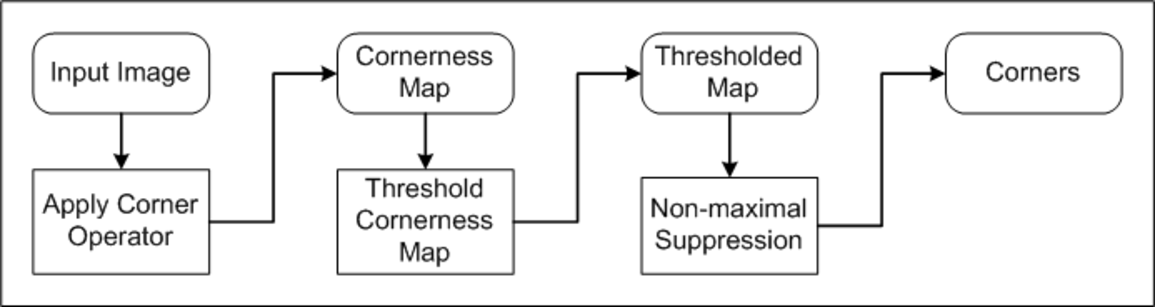
\includegraphics[width=1\columnwidth]{2.mainmatter/1.Introduction/figures/CornerFlowChart}%
\caption[Flowchart for Corner Detectors]{Flowchart for corner detectors.}%
\label{fig:flowchart_corner-detection}%
\end{figure}


\item [\textit{ii. Threshold Cornerness Map:}] The cornerness map is now thresholded to remove the false corners. We set a threshold value that will be able retain true corners.\footnote{Generally, there is no threshold value that can remove all false corner while retaining all true corners. So, the appropriate threshold is dependent on application requirements.}. There is no straightforward method to choose the threshold value, it is application dependent and requires trial and error experimentation~\cite{Parks:11}.
\item [\textit{iii. Non-maximal Suppression:}] The non-maximal suppression is carried out to get the local maxima of the thresholded cornerness map. A distance value is chosen and cornerness measure of all the pixels within the distance will be zero except the largest one. Then the result is cornerness map with non-zero points as corners. 
\end{description}

%Include the theories and basic principles required for image stitching




%\cite{Szeliski:06}
% X-ray images
% Why Image stiching is challenging?
% WorkFlow
% Areas of Application
